\documentclass{beamer}
\usetheme{Boadilla}
\usepackage{hyperref}
\usepackage{graphicx}
\usepackage{fancyvrb}
\usepackage{multicol}
\usepackage{subfig}
\usepackage[
    backend=biber, 
    natbib=true,
    style=numeric,
    sorting=none,
    style=verbose-ibid,
    labelyear
]{biblatex}
\addbibresource{citations.bib}
\usepackage{pgfpages}
\usepackage{xcolor}
\definecolor{ao(english)}{rgb}{0.0, 0.5, 0.0}
\definecolor{burgundy}{rgb}{0.5, 0.0, 0.13}
%\setbeameroption{show notes}
\setbeameroption{show notes on second screen=right}
%\setbeameroption{hide notes}

\title{The Harmonix Set}
\subtitle{Beats, downbeats, and structural annotations for Western pop music}
\author{Sevag Hanssian}
\institute{MUMT 621, Winter 2021}
\setbeamertemplate{navigation symbols}{}

\begin{document}

\begin{frame}
\maketitle
\href{run:./gangnam.wav}{SOUND CHECK}
\end{frame}

\begin{frame}
	\frametitle{The Harmonix Set}
	Abstract \footfullcite{harmonixpaper}, \footfullcite{harmonixrepo}
	\begin{quote}
	The Harmonix set: a collection of annotations of beats, downbeats, and functional segmentation for over 900 full tracks that covers a wide range of western popular music.  Given the variety of annotated music information types in this set, and how strongly these three types of data are typically intertwined,  we seek to foster \textbf{research that focuses on multiple retrieval tasks at once}.
	\end{quote}
\end{frame}

\note{
\begin{itemize}
	\item
		Harmonix is a video game studio -- created Rock Band, among others
\end{itemize}
}

\begin{frame}
	\frametitle{Fundamental MIR tasks}
	\begin{enumerate}
		\item
			Beat tracking\ \\
			MIREX task ``Audio Beat Tracking''\\
			\href{https://www.music-ir.org/mirex/wiki/2006:Audio_Beat_Tracking}{https://www.music-ir.org/mirex/wiki/2006:Audio\_Beat\_Tracking}
		\item
			Downbeat estimation\ \\
			MIREX task ``Audio Downbeat Estimation''\\
			\href{https://www.music-ir.org/mirex/wiki/2014:Audio_Downbeat_Estimation}{https://www.music-ir.org/mirex/wiki/2014:Audio\_Downbeat\_Estimation}
		\item
			Structural segmentation\ \\
			MIREX task ``Structural Segmentation''\\
			\href{https://www.music-ir.org/mirex/wiki/2009:Structural_Segmentation}{https://www.music-ir.org/mirex/wiki/2009:Structural\_Segmentation}
	\end{enumerate}\ \\
	\vspace{2em}
	Often interrelated: downbeats define the first beat of a measure, music segments begin and end on beat (frequently downbeat) locations
\end{frame}

\begin{frame}
	\frametitle{Onset detection, beat tracking, downbeat estimation, structural segmentation}
	The goal of onset detection is finding the time-locations of all sonic events in a piece of audio\footfullcite{onsetmirex}\\
	\vspace{1em}
	The goal of beat tracking is to detect all beat locations in a song, or ``beat instants that might correspond to when a human listener would tap their foot''\footfullcite{ellis07}\\
	\vspace{1em}
	The goal of the related task, downbeat estimation, is to find the first beat of each bar (measure)\\
	\vspace{1em}
	The goal of structural segmentation evaluation is to identify the key structural sections in musical audio
\end{frame}

\note{
	\begin{itemize}
		\item
			Important to note that beat tracking is not necessarily based on, or a subset, of onset detection. Many popular implementations are, though
		\item
			It should be noted that none of the evaluation measures cares about the true labels of the sections: they only denote the clustering. This means that it does not matter if the systems produce true labels such as "chorus" and "verse", or arbitrary labels such as "A" and "B". 
		\item
			corey kereliuk introduction -- foot tapping + chess
	\end{itemize}
}

\begin{frame}
	\frametitle{MIREX beat tracking datasets}
	\begin{enumerate}
		\item[2006]
			First appearance of challenge \footfullcite{beatmeta}; \textit{the MCK dataset contains 160 30-second audio excerpts created by the MIREX team in 2006. Characterized by stable tempo, wide variety of instrumentations and musical styles. 20\% of the files have non-binary meters.}
		\item[2009]
			Second dataset, Chopin Mazurkas\footfullcite{mazurkahard}; \textit{the MAZ dataset contains piano recordings of 322 Chopin Mazurkas, which include tempo changes.}
		\item[2012]
			Third dataset \footfullcite{beats2012}; \textit{consists of 217 excerpts around 40s each, majority is difficult to track (e.g. changes in meter and tempo, bad sound quality, expressive timing). It includes romantic music, film soundtracks, blues, chanson, and solo guitar}
	\end{enumerate}
\end{frame}

\note{
	\begin{itemize}
		\item
			MCK named after McKinney? not really explained, but colloquially looks to be true
		\item
			First dataset is same dataset used in \href{https://www.music-ir.org/mirex/wiki/2006:Audio_Tempo_Extraction}{https://www.music-ir.org/mirex/wiki/2006:Audio\_Tempo\_Extraction}
		\item
			the case study is an important paper. since the HarmonixSet is new, similar assessment hasn't been done yet. goes to show that there are advantages to using well-known datasets, for existing literature
	\end{itemize}
}

\begin{frame}
	\frametitle{MIREX downbeat estimation datasets}
	\begin{enumerate}
		\item[2014]
			Six different datasets from diverse geographic and stylistic sources:
			\textbf{The Beatles} \footcite{beatles}, \textbf{HJDB} \footcite{hjdb} (Hardcore, Jungle, Drum and Bass)
			\textbf{Turkish} \footcite{turkish}, \textbf{Ballroom} \footcite{ballroom}
			\textbf{Carnatic} \footcite{carnatic}, \textbf{Cretan} \footcite{cretan}
	\end{enumerate}
\end{frame}

\note{
	\begin{itemize}
		\item
			Interesting trend, in beat tracking, MIREX supplied the dataset
		\item
			In downbeat estimation, the datasets are gathered from BYO-dataset per paper
	\end{itemize}
}

\begin{frame}
	\frametitle{MIREX structural segmentation datasets}
	MIREX datasets:
	\begin{enumerate}
		\item
			\textbf{The Beatles} (same as beat/downbeat Beatles dataset) \footcite{beatles}
		\item
			Subset of \textbf{RWC} \footcite{rwc}
		\item
			Evolution of The Beatles dataset, \textbf{Isophonics Dataset}\footcite{isophonics}
	\end{enumerate}
	Difficult traits of structural segmentation:
	\begin{enumerate}
		\item
			Ambiguous -- more than one valid annotation for a given track
		\item
			Subjective -- different listeners can perceive different segments
	\end{enumerate}
	Solutions: SALAMI\footcite{salami}, SPAM\footcite{spam} (multiple annotations per track by different experts), which also introduce hierarchical segments
\end{frame}

\note{
	\begin{itemize}
		\item
			Difference from beat/downbeat annotations: cannot have excerpts, need whole song
		\item
			Hierarchical vs flat segments
	\end{itemize}
}

\begin{frame}
	\frametitle{Dataset annotators}
\end{frame}

\begin{frame}
	\frametitle{MIREX vs. HarmonixSet results}
\end{frame}


\begin{frame}[fragile]
	\frametitle{Gangnam style -- HarmonixSet annotations}
	\begin{enumerate}
		\item
		\begin{verbatim}
		# dataset/beats_and_downbeats/0388_gangnamstyle.txt
		0.079   1       1
		0.54    2       1
		1.017   3       1
		1.494   4       1
		1.92    1       2
		2.374545        2       2
		2.82909 3       2
		3.283635        4       2
		\end{verbatim}
		\item
		\begin{verbatim}
		# dataset/segments/0388_gangnamstyle.txt
		0.079    intro
		6.010905 chorus
		14.64726 verse
		\end{verbatim}
		\item
		\href{https://github.com/urinieto/harmonixset/blob/master/dataset/jams/0388_gangnamstyle.jams}{https://github.com/urinieto/harmonixset/blob/master/dataset/jams/0388\_gangnamstyle.jams}\footfullcite{jams}
	\end{enumerate}

\end{frame}

\begin{frame}[fragile]
	\frametitle{Gangnam style results -- beats}
	Beat time output from INSERTURLHERE\footfullcite{madmombeats}
	\begin{verbatim}
	beat times: [ 0.09  0.55  1. 1.46 1.91 2.37 2.82 3.28 ... ]
	\end{verbatim}
	vs. HarmonixSet ground truth
	\begin{verbatim}
	# dataset/beats_and_downbeats/0388_gangnamstyle.txt
	0.079   1       1
	0.54    2       1
	1.017   3       1
	1.494   4       1
	1.92    1       2
	2.374545        2       2
	2.82909 3       2
	3.283635        4       2
	\end{verbatim}
	Clicks: \href{run:./gangnam_beats.wav}{BEAT CLICKS}
\end{frame}

\begin{frame}[fragile]
	\frametitle{Gangnam style results -- downbeats}
	Downbeat time output from INSERTURLHERE\footfullcite{madmomdownbeats}
	\begin{verbatim}
	downbeat times: [1.0, 2.82, 4.64, 6.46, ...]
	\end{verbatim}
	vs. HarmonixSet ground truth (\textbf{NB!} not first beat of bar, but consistently lands on third)
	\begin{verbatim}
	# awk '{ if ($2 == 3) { print }}' \
	#     dataset/beats_and_downbeats/0388_gangnamstyle.txt
	1.017   3       1
	2.82909 3       2
	4.64727 3       3
	6.46545 3       4
	...
	\end{verbatim}
	Clicks: \href{run:./gangnam_downbeats.wav}{DOWNBEAT CLICKS}
\end{frame}

\begin{frame}[fragile]
	\frametitle{Gangnam style results -- segmentation}
	Structural segmentation output from INSERTURLHERE\footfullcite{librosaseg}
	\begin{verbatim}
	segments: [ 0.58049887  7.87156463  8.82358277 12.63165533
	      	    14.90721088 16.27718821 19.99238095]
	\end{verbatim}
	vs. HarmonixSet ground truth
	\begin{verbatim}
	0.079 intro, 6.010905 chorus, 14.64726 verse
	\end{verbatim}
	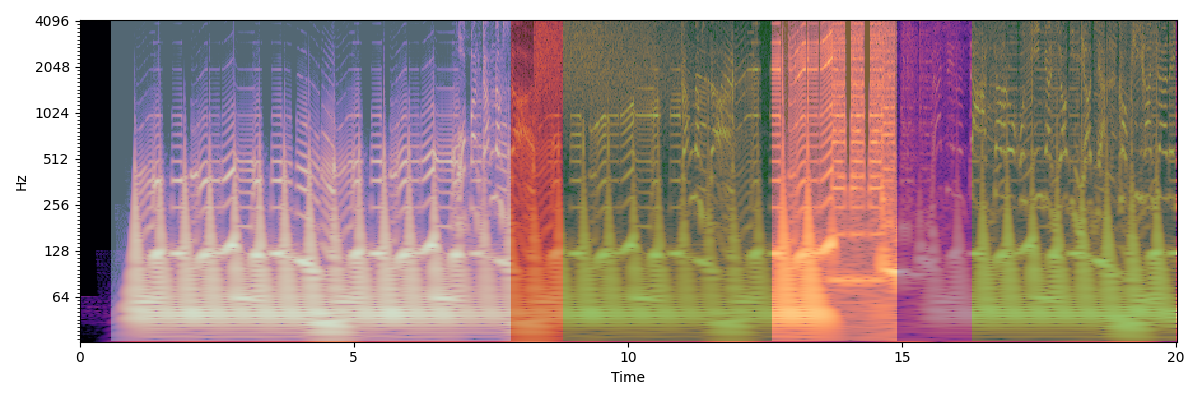
\includegraphics[width=9.5cm]{./laplacian_segments.png}\\
	\href{run:./gangnam_segments.wav}{SEGMENT PAUSES}, \href{run:./gangnam_segments_truth.wav}{TRUTH SEGMENT PAUSES}
\end{frame}

\begin{frame}
	\frametitle{Audio alignment}
	YouTube music video, or different file formats or recordings obtained by researchers, may have temporal differences with the original mp3 files. Alignment data is included to
	\begin{quote}
	... help align the audio in case researchers obtain audio data with different compression formats that might include certain small temporal offsets.
	\end{quote}
	Algorithms used for alignment:
	\begin{enumerate}
		\item
			Dynamic time warping \footfullcite{dtw}, \footfullcite{dtwnotebook}
		\item
			Onsets \footfullcite{librosaonset}
	\end{enumerate}
\end{frame}

\note{
\begin{itemize}
	\item
		DTW in a nutshell:
		\begin{quote}
		DTW has been successfully applied to automatically cope with time deformations and different speeds associated with time-dependent data.
		\end{quote}
	\item
		Onsets don't quite solve the problem, unlike DTW. They're just timestamped information. One would have to do some manual work to compare their onsets to the harmonixset onsets and compute the temporal difference -- or perhaps it can be used as an indicator to run DTW
\end{itemize}
}

\begin{frame}[fragile]
	\frametitle{Gangnam style temporal alignment -- onsets}
	Onset output from INSERTURLHERE\footfullcite{librosaonset}
	\begin{verbatim}
	onset times: [ 1.01006803  1.46285714  1.69505669 
	       1.92725624  2.04335601  2.38004535
	       2.6122449   2.83283447  3.29723356 ...
	\end{verbatim}
	vs. HarmonixSet onsets from JAMS file from INSERTURLHERE
	\begin{verbatim}
	# ./jams_onsets.py dataset/jams/0388_gangnamstyle.jams
	0.139 0.604 0.813 1.068 1.184 1.509 1.95
	2.415 2.647 2.879 3.088 ...
	\end{verbatim}
	Clicks: \href{run:./gangnam_onsets.wav}{ONSET CLICKS}
\end{frame}

\note{
	\begin{itemize}
		\item
			I tried librosa 0.8.0, 0.7.0, default onset parameters, same as harmonixset -- strange mismatch in onset values. Should report
	\end{itemize}
}

\begin{frame}
	\frametitle{Dataset recreation and copyright}
	Data provided to allow independent recreation of dataset includes:\\
	Identifiers in shared music databases:
	\begin{enumerate}
		\item
			MusicBrainz ID \footfullcite{musicbrainz}, open music encyclopedia including unique identifiers for recordings, releases, artists, etc.
		\item
			AcoustID (\href{https://acoustid.org/}{https://acoustid.org/}), open source fingerprinting service to easily match audio content associated with MusicBrainz ids
		\item
			YouTube URLs, including alignment information with the original mp3 files used in the paper
	\end{enumerate}
	Audio/DSP features:
	\begin{enumerate}
		\item
			mel spectrograms for the original mp3 files
		\item
			estimated onsets for the first 30 seconds of audio from librosa
	\end{enumerate}
\end{frame}

\note{
\begin{itemize}
	\item
		Original mp3 files cannot legally be distributed due to copyright
	\item
		Note that these audio features are automated (onsets and spectrograms). This allows independent recreation (aligning the direct output of librosa's onset function on my files and comparing it to their's)
	\item
		Keep in mind onsets are (most likely) essential in beat/downbeat/segmentation tracking. note onsets mark musical events, its a fact. but the raw librosa onset data isn't the opinionated ``algorithm being evaluated'', in this sense its used as a straight feature
\end{itemize}
}

\end{document}
